\begin{tikzpicture}
  \GraphInit[vstyle=Classic]

  \Vertex{v}
  \Vertex[a=0, d=3cm, L=$y_{1}$]{y1}
  \Vertex[a=25, d=3cm, L=$y_{2}$]{y2}
  \Vertex[a=50, d=3cm, L=$y_{3}$]{y3}
  \Vertex[a=85, d=3cm, L=$y_{i-1}$]{yim1}
  \Vertex[a=110, d=3cm, L=$y_{i}$]{yi}

  \Edge[style ={-, dashed}]({v})({y1})
  \Edge[style ={-}, label={$t_{1}$},labelstyle={above}]({v})({y2})
  \Edge[style ={-}, label={$t_{2}$},labelstyle={above}]({v})({y3})
  \Edge[style ={-}, label={$t_{i - 2}$},labelstyle={above}]({v})({yim1})
  \Edge[style ={-}, label={$t_{i - 1}$},labelstyle={above}]({v})({yi})
 
\end{tikzpicture}

